\subsection{R1: long video rollout}
The paper's Figure 3 compares video models, and Figures 8--9 illustrate Minecraft rollout beyond its recurrent training horizon. The source uses the same image file for Figures 8 and 9. We completed one-, two- and eight-times autoregressive runs, each containing eight videos with two context frames. The eight-times run generated 80-frame clips in 102.2 minutes, using a sampled peak of 14,343 MiB VRAM. The four-times horizon and the alternative schedule remain pending.

Within the eight-times run, generated-transition LPIPS was $0.1339\pm0.0397$ over the first training horizon and $0.1366\pm0.0566$ over the last (standard deviations across video means); its fitted slope was $8.47\times10^{-5}$ per frame. MSE increased from $0.01450\pm0.00679$ to $0.01780\pm0.00963$. Ground-truth late-horizon means were 0.1382 LPIPS and 0.01415 MSE. Mean intensity across generated frames ranged from 0.3326 to 0.4128, and mean within-frame pixel standard deviation from 0.2516 to 0.2923. These aggregate statistics and the reviewed filmstrips show no gross saturation or complete freezing in this sample, although they do not rule out artifacts in individual videos. The result provides limited support for stable long rollout under the released checkpoint; it does not establish equivalence to the paper's model or baselines.

The two-times run yielded late-horizon MSE $0.01044\pm0.00550$ and LPIPS $0.1248\pm0.0614$. The separate one-times run yielded MSE $0.01313\pm0.00648$ and LPIPS $0.1433\pm0.0543$. Dataset window enumeration changes with horizon, so the one- and eight-times batches are not paired. The within-run early/late comparison above avoids treating them as paired observations. All tensors were finite; eight-times predictions ranged from $-0.1861$ to $1.2999$ before clamping to $[0,1]$ for metrics.

This experiment reproduces only DF's portion of the comparison: the released quickstart does not provide the teacher-forcing and causal full-sequence baselines. The attention checkpoint's sliding window and 110,000 steps recorded in its checkpoint (100,000 in the README) differ from the paper's RNN. Minecraft futures are stochastic; frame-to-frame change measures stability rather than predictive accuracy. A flat, nonzero curve near ground-truth change is consistent with no divergence, while a curve approaching zero can indicate freezing rather than stability. Evidence is limited to one sampling seed and eight videos.

\begin{figure}[ht]
\centering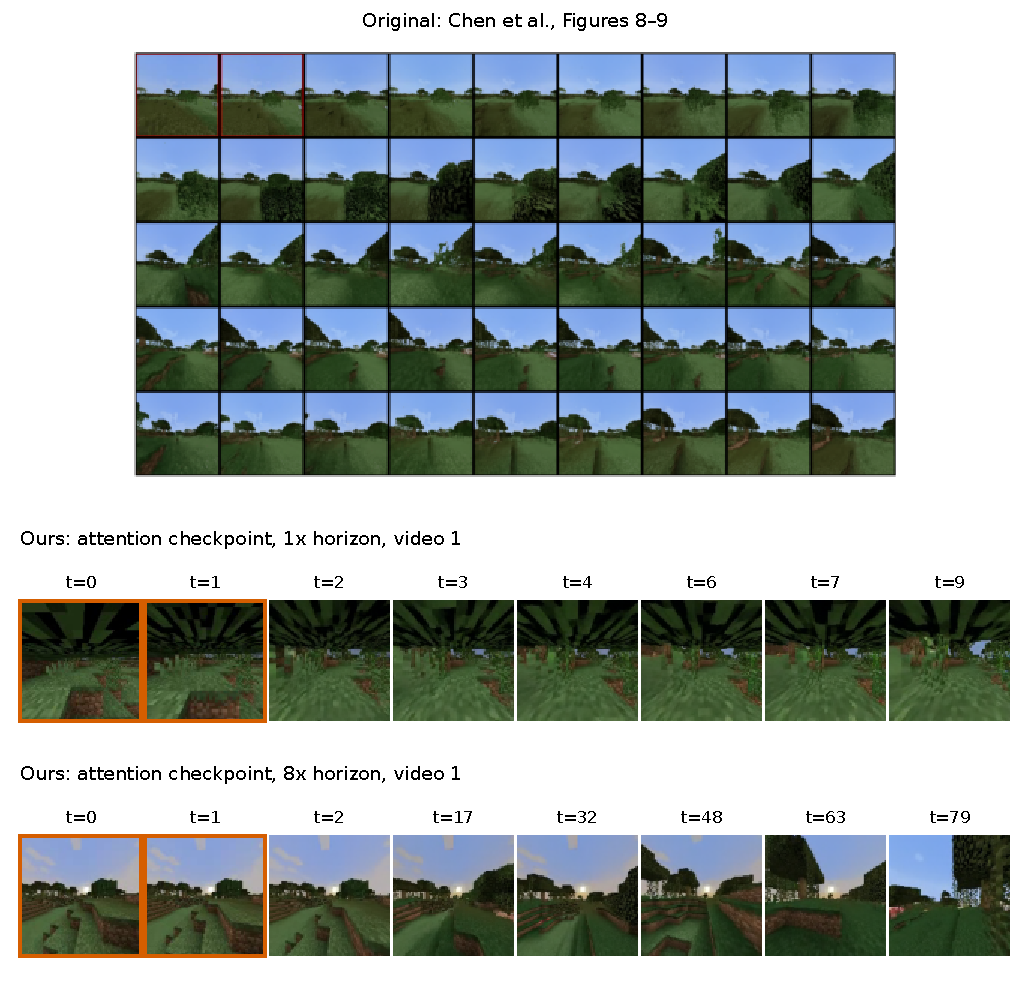
\includegraphics[width=\linewidth]{figures/r1_minecraft_compare.pdf}
\caption{Top (original, Chen et al., Figures 8--9): Minecraft rollout from the paper's recurrent model, reproduced from the paper source. Middle and bottom (ours): released attention checkpoint at one and eight times its configured training horizon. Orange borders identify context frames. Architectures, rollout mechanisms and input clips differ.}
\end{figure}
\begin{figure}[ht]
\centering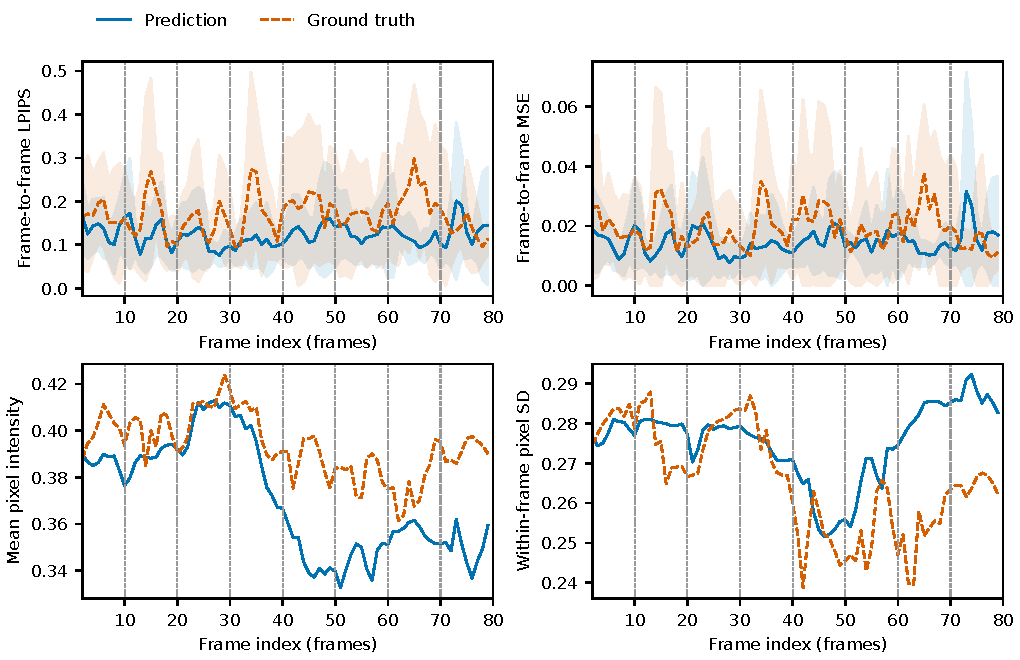
\includegraphics[width=\linewidth]{figures/r1_temporal_metrics.pdf}
\caption{Ours: eight-times autoregressive rollout, with matched ground-truth temporal-change reference. Lines average eight videos; shaded regions in the LPIPS and MSE panels are one standard deviation across videos, not confidence intervals. Dashed vertical lines mark ten-frame training-horizon boundaries. Pixel statistics use clamped $[0,1]$ values.}
\end{figure}
\subsection{R2: planning audit, experiments pending}
The release explicitly changes the planning setting and omits MCG (called MCTG in the README). Exact Table 1 reproduction is therefore not available from the permitted \texttt{main} workflow. The asterisk on Diffuser denotes a hand-crafted PD controller that ignores generated actions, not merely a matched evaluation setting. Paper single-task means are shown next to explicitly missing released-code results.
\begin{table}[ht]
\centering
\begin{tabular}{lrrlll}
\toprule
Maze & Paper DF & Paper Diffuser* & Ours reward & Ours stay & Ours reach\\
\midrule
Medium & 149.4 & 121.5 & TBD & TBD & TBD\\
Large & 159.0 & 123.0 & TBD & TBD & TBD\\
\bottomrule
\end{tabular}
\caption{Left numeric columns: original Table 1, Chen et al. Right three columns: our planned released-main evaluation, not yet run. Paper values are historical context, not directly comparable to raw released-code metrics. ``Stay'' denotes reward-if-stay and ``reach'' denotes first-reach steps.}
\end{table}
The code's \texttt{episode\_reward} is closest in construction to accumulated episode reward; \texttt{episode\_reward\_if\_stay} changes the trajectory outcome by crediting every step after first success. Neither can be compared numerically to paper scores without verifying normalization and evaluation protocol. The implementation increments \texttt{first\_reach} only while the goal has not yet been reached, excluding the successful step, and non-reaching episodes are censored at the evaluated duration. The analysis also records reached flags. MuJoCo 2.1.0 and D4RL now import successfully, and medium/large environments pass two-environment reset/step checks through the planner's vector interface. This verifies setup only; policy evaluation is queued after video sampling. Original planning Figures 14--15 are available in the source, but our corresponding plans are \textbf{[TBD]}.
\subsection{R3: expanded theoretical result}
\begin{table}[ht]
\centering
\begin{tabular}{p{0.44\linewidth}p{0.44\linewidth}}
\toprule
Original Appendix A (v4) & Our algebraic audit\\
\midrule
Claim 3 assigns positive KL to the expected log ratio $\mathbb E_q\log(p/q)$. & The identity is $-D_{\rm KL}(q\Vert p)$; the corrected lower bound subtracts denoising errors.\\
Equation (A.13) counts uniform noise levels. & Explicit counting yields $1/(K+1)$ and $(j+1)/(K+1)$.\\
Theorem A.3 uses $jP_t(j\mid k_{<t})$. & General weights are $\Pr(k_t<j\mid k_{<t})$; the forms coincide for uniform levels, but not generally.\\
\bottomrule
\end{tabular}
\caption{Left: original paper statements, paraphrased from Appendix A. Right: our derivation and corrections. This analytical comparison is completed; it complements the experimental R1 result.}
\end{table}
\paragraph{R3: audited statement and notation.}
We expand Appendix A of arXiv:2407.01392v4 \cite{chen2025diffusion}. This is a corrected derivation of the intended ELBO, not a verification of every displayed formula as printed. In particular, Claim 3 prints $\mathbb E_q\log(p/q)=D_{\rm KL}(q\Vert p)$; the correct sign is negative. Theorem A.1 also reverses the arguments of the model transition in its KL. The derivation below consistently uses the reverse transition $p_\theta(x^{j-1}\mid x^j,z)$. Equation (A.13) is an indicator-expectation identity, not the Gaussian KL identity.

Let $x^0_{1:T}$ be a fixed clean sequence, with token dimension $d$, and let $k_t\in\{0,\ldots,K\}$ be independent uniform noise levels. For each token, $q(x^{1:K}\mid x^0)=\prod_{j=1}^Kq(x^j\mid x^{j-1})$ is the forward Markov chain. Write $y_t=x_t^{k_t}$ and let $z_t=z_t(k_{1:t})$ summarize the noisy history; indexing the latent by the noise history avoids assigning conflicting values to one latent variable. The model satisfies $p_\theta(y_t,z_t\mid y_{<t},z_{<t})=p_\theta(y_t,z_t\mid z_{t-1})$. Its token-level reverse chain is
\[
 p_\theta(x^{k:K}\mid z)=r(x^K)\prod_{j=k+1}^Kp_\theta(x^{j-1}\mid x^j,z),
\]
where the terminal prior $r$ is fixed and independent of $z$ and $\theta$. As in the paper, assume these conditionals arise from a consistent joint probability measure on the noise-level copies and history-indexed latents. For a fixed noise vector, $p_\theta(y_{1:T})$ denotes its selected marginal, not a mixture over noise vectors. $\mathbb E_{\rm forward}$ includes the stated draw of noise levels as well as the forward-chain variables; other expectations include the relevant chain variables even when only a marginal is displayed. Assume the densities and logarithms are integrable; otherwise the lower bound may be $-\infty$.

\paragraph{Paper Claim 1: expanding the latents.}
Define $Q_z=\prod_t p_\theta(z_t\mid z_{t-1},y_t)$. Factoring the joint distribution gives
\[
 p_\theta(y_{1:T})=\mathbb E_{Q_z}\prod_{t=1}^T p_\theta(y_t\mid z_{t-1}),\qquad
 \log p_\theta(y_{1:T})\geq\mathbb E_{Q_z}\sum_t\log p_\theta(y_t\mid z_{t-1}).
\]
\emph{Expanded step:} $Q_z$ is a normalized sequential distribution, not necessarily the full posterior conditioned on all observations. The inequality is Jensen's inequality for the concave logarithm. Deterministic latent updates make the product constant under $Q_z$, giving equality. Averaging over the forward process reduces the problem to bounding each token likelihood conditional on its sampled past.

\paragraph{Paper Claim 2: importance sampling and Jensen.}
Fix $t,k,z=z_{t-1}$, put $y=x_t^k$, $u=x_t^{k+1:K}$ and $Q(u\mid y)=q(u\mid y)$. Then
\begin{align*}
 p_\theta(y\mid z)&=\int p_\theta(y,u\mid z)\,du
 =\mathbb E_{Q(u\mid y)}\frac{p_\theta(y,u\mid z)}{Q(u\mid y)},\\
 \log p_\theta(y\mid z)&\geq
 \mathbb E_Q\left[\log p_\theta(y,u\mid z)-\log Q(u\mid y)\right]
 =:\mathcal L_k(y,z).
\end{align*}
\emph{Expanded step:} the importance-sampling equality requires the model measure on $u$ to be absolutely continuous with respect to $Q$: no model mass may lie where $Q=0$. Nondegenerate Gaussian chains satisfy this. A finite ELBO also requires $Q$ not to put positive mass where the model density is zero. Concavity gives $\log\mathbb E_Q W\geq\mathbb E_Q\log W$. More explicitly,
\[
 \log p_\theta(y\mid z)-\mathcal L_k(y,z)
 =D_{\rm KL}\bigl(Q(u\mid y)\Vert p_\theta(u\mid y,z)\bigr)\geq0.
\]
Thus equality requires an exact variational posterior. When $k=K$, $u$ is empty and this step is an equality. These are the paper's two Jensen inequalities, including the latent step above.

\paragraph{Paper Claim 3: time reversal and telescoping.}
For $k\geq1$, Bayes' rule and the forward Markov property give
\[
 q(x^j\mid x^{j-1})=
 q(x^{j-1}\mid x^j,x^0)\frac{q(x^j\mid x^0)}{q(x^{j-1}\mid x^0)}.
\]
\emph{Expanded step:} this follows by expressing the same conditional joint density of $(x^{j-1},x^j)$ given $x^0$ in both orders. Substituting it into the log likelihood ratio produces the marginal-density sum
\begin{align*}
 &\bigl[\log q(x^k\mid x^0)-\log q(x^{k+1}\mid x^0)\bigr]\\
 &+\bigl[\log q(x^{k+1}\mid x^0)-\log q(x^{k+2}\mid x^0)\bigr]+\cdots\\
 &+\bigl[\log q(x^{K-1}\mid x^0)-\log q(x^K\mid x^0)\bigr]\\
 &=\log q(x^k\mid x^0)-\log q(x^K\mid x^0).
\end{align*}
Every intermediate marginal cancels. Consequently, after taking the forward expectation,
\[
 \mathbb E_q\mathcal L_k=C_k(x^0)
 -\sum_{j=k+1}^K\mathbb E_{q(x^j\mid x^0)}
 D_{\rm KL}\bigl(q(x^{j-1}\mid x^j,x^0)\Vert
 p_\theta(x^{j-1}\mid x^j,z)\bigr),\quad k\geq1,
\]
where $C_k=\mathbb E_q[\log r(x^K)-\log q(x^K\mid x^0)+\log q(x^k\mid x^0)]$ is parameter independent. This also handles $k=K$ with an empty sum. For $k=0$, the clean endpoint is fixed, so one must keep the reconstruction term instead of using a density for a Dirac mass:
\[
 \mathbb E_q\mathcal L_0=C_0(x^0)+\mathbb E_q\log p_\theta(x^0\mid x^1,z)
 -\sum_{j=2}^K\mathbb E_{q(x^j\mid x^0)}D_{\rm KL}(q(x^{j-1}\mid x^j,x^0)\Vert p_\theta(x^{j-1}\mid x^j,z)),
\]
with $C_0=\mathbb E_q[\log r(x^K)-\log q(x^K\mid x^0)]$. These signs follow directly from $\int q\log(p/q)=-D_{\rm KL}(q\Vert p)$.

\paragraph{Equation (A.13), expanded.}
There is one choice $k=0$ out of $K+1$ possibilities. For $0\leq j<K$, the event $k\leq j$ contains $j+1$ possibilities, so
\[
 \mathbb E\mathbf1\{k=0\}=\frac1{K+1},\qquad
 \mathbb E\mathbf1\{j\geq k\}=\sum_{k=0}^j\frac1{K+1}=\frac{j+1}{K+1}.
\]
A reverse transition from $j$ to $j-1$ appears whenever $k<j$, hence has weight $j/(K+1)$. Combining the three claims yields the corrected intended statement
\begin{align*}
 \mathbb E_{\rm forward}\log p_\theta(y_{1:T})\geq C+
 \sum_t\mathbb E_{<t}\biggl[&\frac{1}{K+1}\mathbb E_q\log p_\theta(x_t^0\mid x_t^1,z_{t-1})\\
 &-\sum_{j=2}^K\frac{j}{K+1}\mathbb E_{q(x_t^j\mid x_t^0)}D_{t,j}\biggr],
\end{align*}
where $D_{t,j}$ is the reverse-transition KL above and $\mathbb E_{<t}$ averages noisy history and latent updates. In contrast to the printed positive-KL expression, improving a denoiser increases this lower bound.

\paragraph{Expanded Gaussian KL reduction.}
Let $q(x^j\mid x^{j-1})=\mathcal N(\sqrt{\alpha_j}x^{j-1},\beta_j I)$, $\alpha_j=1-\beta_j$, and $\bar\alpha_j=\prod_{i=1}^j\alpha_i$. Completing the square in
$q(x^j\mid x^{j-1})q(x^{j-1}\mid x^0)$ gives posterior variance and mean
\[
 \widetilde\beta_j=\frac{\beta_j(1-\bar\alpha_{j-1})}{1-\bar\alpha_j},\qquad
 \widetilde\mu_j=A_jx^j+B_jx^0,
\]
\[
 A_j=\frac{\sqrt{\alpha_j}(1-\bar\alpha_{j-1})}{1-\bar\alpha_j},\qquad
 B_j=\frac{\beta_j\sqrt{\bar\alpha_{j-1}}}{1-\bar\alpha_j}.
\]
Indeed, the posterior precision is $\alpha_j/\beta_j+1/(1-\bar\alpha_{j-1})=1/\widetilde\beta_j$; multiplying its inverse by the linear coefficient gives the displayed mean. For $j\geq2$, take model covariance $\sigma_j^2I>0$, fixed independently of $\theta$, and model mean $A_jx^j+B_j\widehat x^0_\theta$. The Gaussian KL is
\[
 D_{t,j}=\frac12\left[d\left(\frac{\widetilde\beta_j}{\sigma_j^2}-1+\log\frac{\sigma_j^2}{\widetilde\beta_j}\right)
 +\frac{B_j^2}{\sigma_j^2}\|\widehat x^0_\theta-x^0\|^2\right].
\]
The first term is parameter independent. Thus $c_j=B_j^2/(2\sigma_j^2)$ multiplies the squared error, and $j/(K+1)$ supplies the additional partial-noise weight. At $j=1$, use a separate finite-variance Gaussian decoder; its negative log likelihood is a constant plus $\|\widehat x^0-x^0\|^2/(2\sigma_1^2)$. Setting its variance to the degenerate forward posterior variance would be invalid.

Writing $x^j=\sqrt{\bar\alpha_j}x^0+\sqrt{1-\bar\alpha_j}\epsilon$, consistent parameterizations give
\[
 \|\widehat x^0-x^0\|^2=\frac{1-\bar\alpha_j}{\bar\alpha_j}\|\widehat\epsilon-\epsilon\|^2
 =(1-\bar\alpha_j)\|\widehat v-v\|^2,
\]
where $v=\sqrt{\bar\alpha_j}\epsilon-\sqrt{1-\bar\alpha_j}x^0$ and $x^0=\sqrt{\bar\alpha_j}x^j-\sqrt{1-\bar\alpha_j}v$. These identities supply the corresponding loss weights without changing the ELBO sign.

\paragraph{Expanded subsequence marginalization.}
Let $S\subseteq\{1,\ldots,T\}$ be the observed token indices. Set $k_t=0$ for $t\in S$ and $k_t=K$ otherwise. Under exact terminal masking, the omitted forward tokens $u=(x_t^K)_{t\notin S}$ have a data-independent density $r_S(u)=\prod_{t\notin S}r(x_t^K)$. For the consistent joint measure assumed above,
\begin{align*}
\log p_\theta(x_S^0)
 &=\log\mathbb E_{r_S}\frac{p_\theta(x_S^0,u)}{r_S(u)}\\
 &\geq\mathbb E_{r_S}\log p_\theta(x_S^0,u)-\mathbb E_{r_S}\log r_S(u).
\end{align*}
The importance-sampling support condition is the same as before. This additional Jensen step has gap
$D_{\rm KL}(r_S(u)\Vert p_\theta(u\mid x_S^0))$; the noise-entropy term is independent of $\theta$. Applying the fixed-noise-vector bound to its right-hand side gives an ELBO for the subsequence marginal. Observed tokens retain every denoising level, while fully masked tokens contribute no reverse-transition loss. These token/history combinations are covered by independent-noise training, up to the sufficient-capacity and endpoint qualifications below. For $S=\{1,\ldots,T\}$ the omitted variables are empty, recovering the full clean-sequence case. This argument assumes consistent marginals; an arbitrary collection of separately specified conditional networks does not establish that assumption on its own.

\paragraph{Subsequences and limits of the guarantee.}
For an arbitrary distribution of noise histories, the coefficient on reverse step $j$ is $\Pr(k_t<j\mid k_{<t})$, and the decoder coefficient is $\Pr(k_t=0\mid k_{<t})$. They are cumulative probabilities, not generally $j\Pr(k_t=j\mid k_{<t})$ as printed in Theorem A.3. Clean tokens and completely masked tokens represent subsequence observations when terminal noise is independent of clean data; finite Gaussian schedules with nonzero terminal signal only approximate complete masking. Independent-noise training covers these histories. Dropping the weights preserves simultaneous optima only under the paper's idealized sufficient-capacity assumptions; it need not do so for a finite shared network. The bound is on expected log likelihood of partially noised sequences, not a proof of rollout stability or of tightness for a trained checkpoint. The released base configuration uses \texttt{noise\_level: random\_all}; its implementation draws indices from $0$ through $999$ for $1000$ diffusion steps. Code index zero is the first positive-noise step, rather than the theorem's exactly clean endpoint $k=0$. Video additionally uses fused-SNR weighting and a finite attention window. Our inference-only audit therefore establishes a connection to the training principle, not empirical verification of the theorem's idealized assumptions.

